The electronics employed to characterize the S13360-6075 SiPM from \newline Hamamatsu is described in this appendix. This electronics consists of three different PCBs connected through HDMI connectors:

\begin{enumerate}
\item{} In the first PCB, shown in Figure \ref{fig:PCB1}, up to 8 SiPMs and one temperature sensor are connected. This PCB is placed inside a light-tight box from Thorlabs \cite{ThorlabsCompany}. This black box has a small hole of $1~\mm$ diameter prepared to introduce an optical fibre\footnote{The optical fibre used is BCF-98 from Saint-Gobain \cite{OpticalFibers}} to illuminate SiPMs with a 430L LED from Thorlabs \cite{LEDThorlabs}. The spectrum of this LED, shown in Figure \ref{fig:LEDSpectrum}, was measured with a spectrometer. The emission peak is located at $436~\nm$ with an FWHM of $19~\nano\meter$. With the help of this LED, the light emission of the TRITIUM scintillating fibres was simulated to calibrate the SiPMs at the working wavelength. 

\item{} In the second PCB, shown in Figure \ref{fig:PCB2}, the signals of the SiPMs are summed and amplified by a factor of either $G=4187$ or $G=10761$, depending on the input resistance of the oscilloscope, $50~\ohm$ or $1~\mega\ohm$ respectively. This PCB includes a differential amplifier to reduce the electronic noise of the system.

\item{} In the third PCB, shown in Figure \ref{fig:PCB3}, the different input and output signals are rearranged to avoid crosstalk. The input signals are the supply voltage of the SiPMs and the PCBs ($\pm 6~\volt$) and the output signals are the temperature sensor signal and the sum of the SiPM signals. The output signal of the third PCB is recorded by an MSO44X oscilloscope from Tektronix \cite{Oscilloscope}.

\end{enumerate}

\begin{figure}[h]
\centering
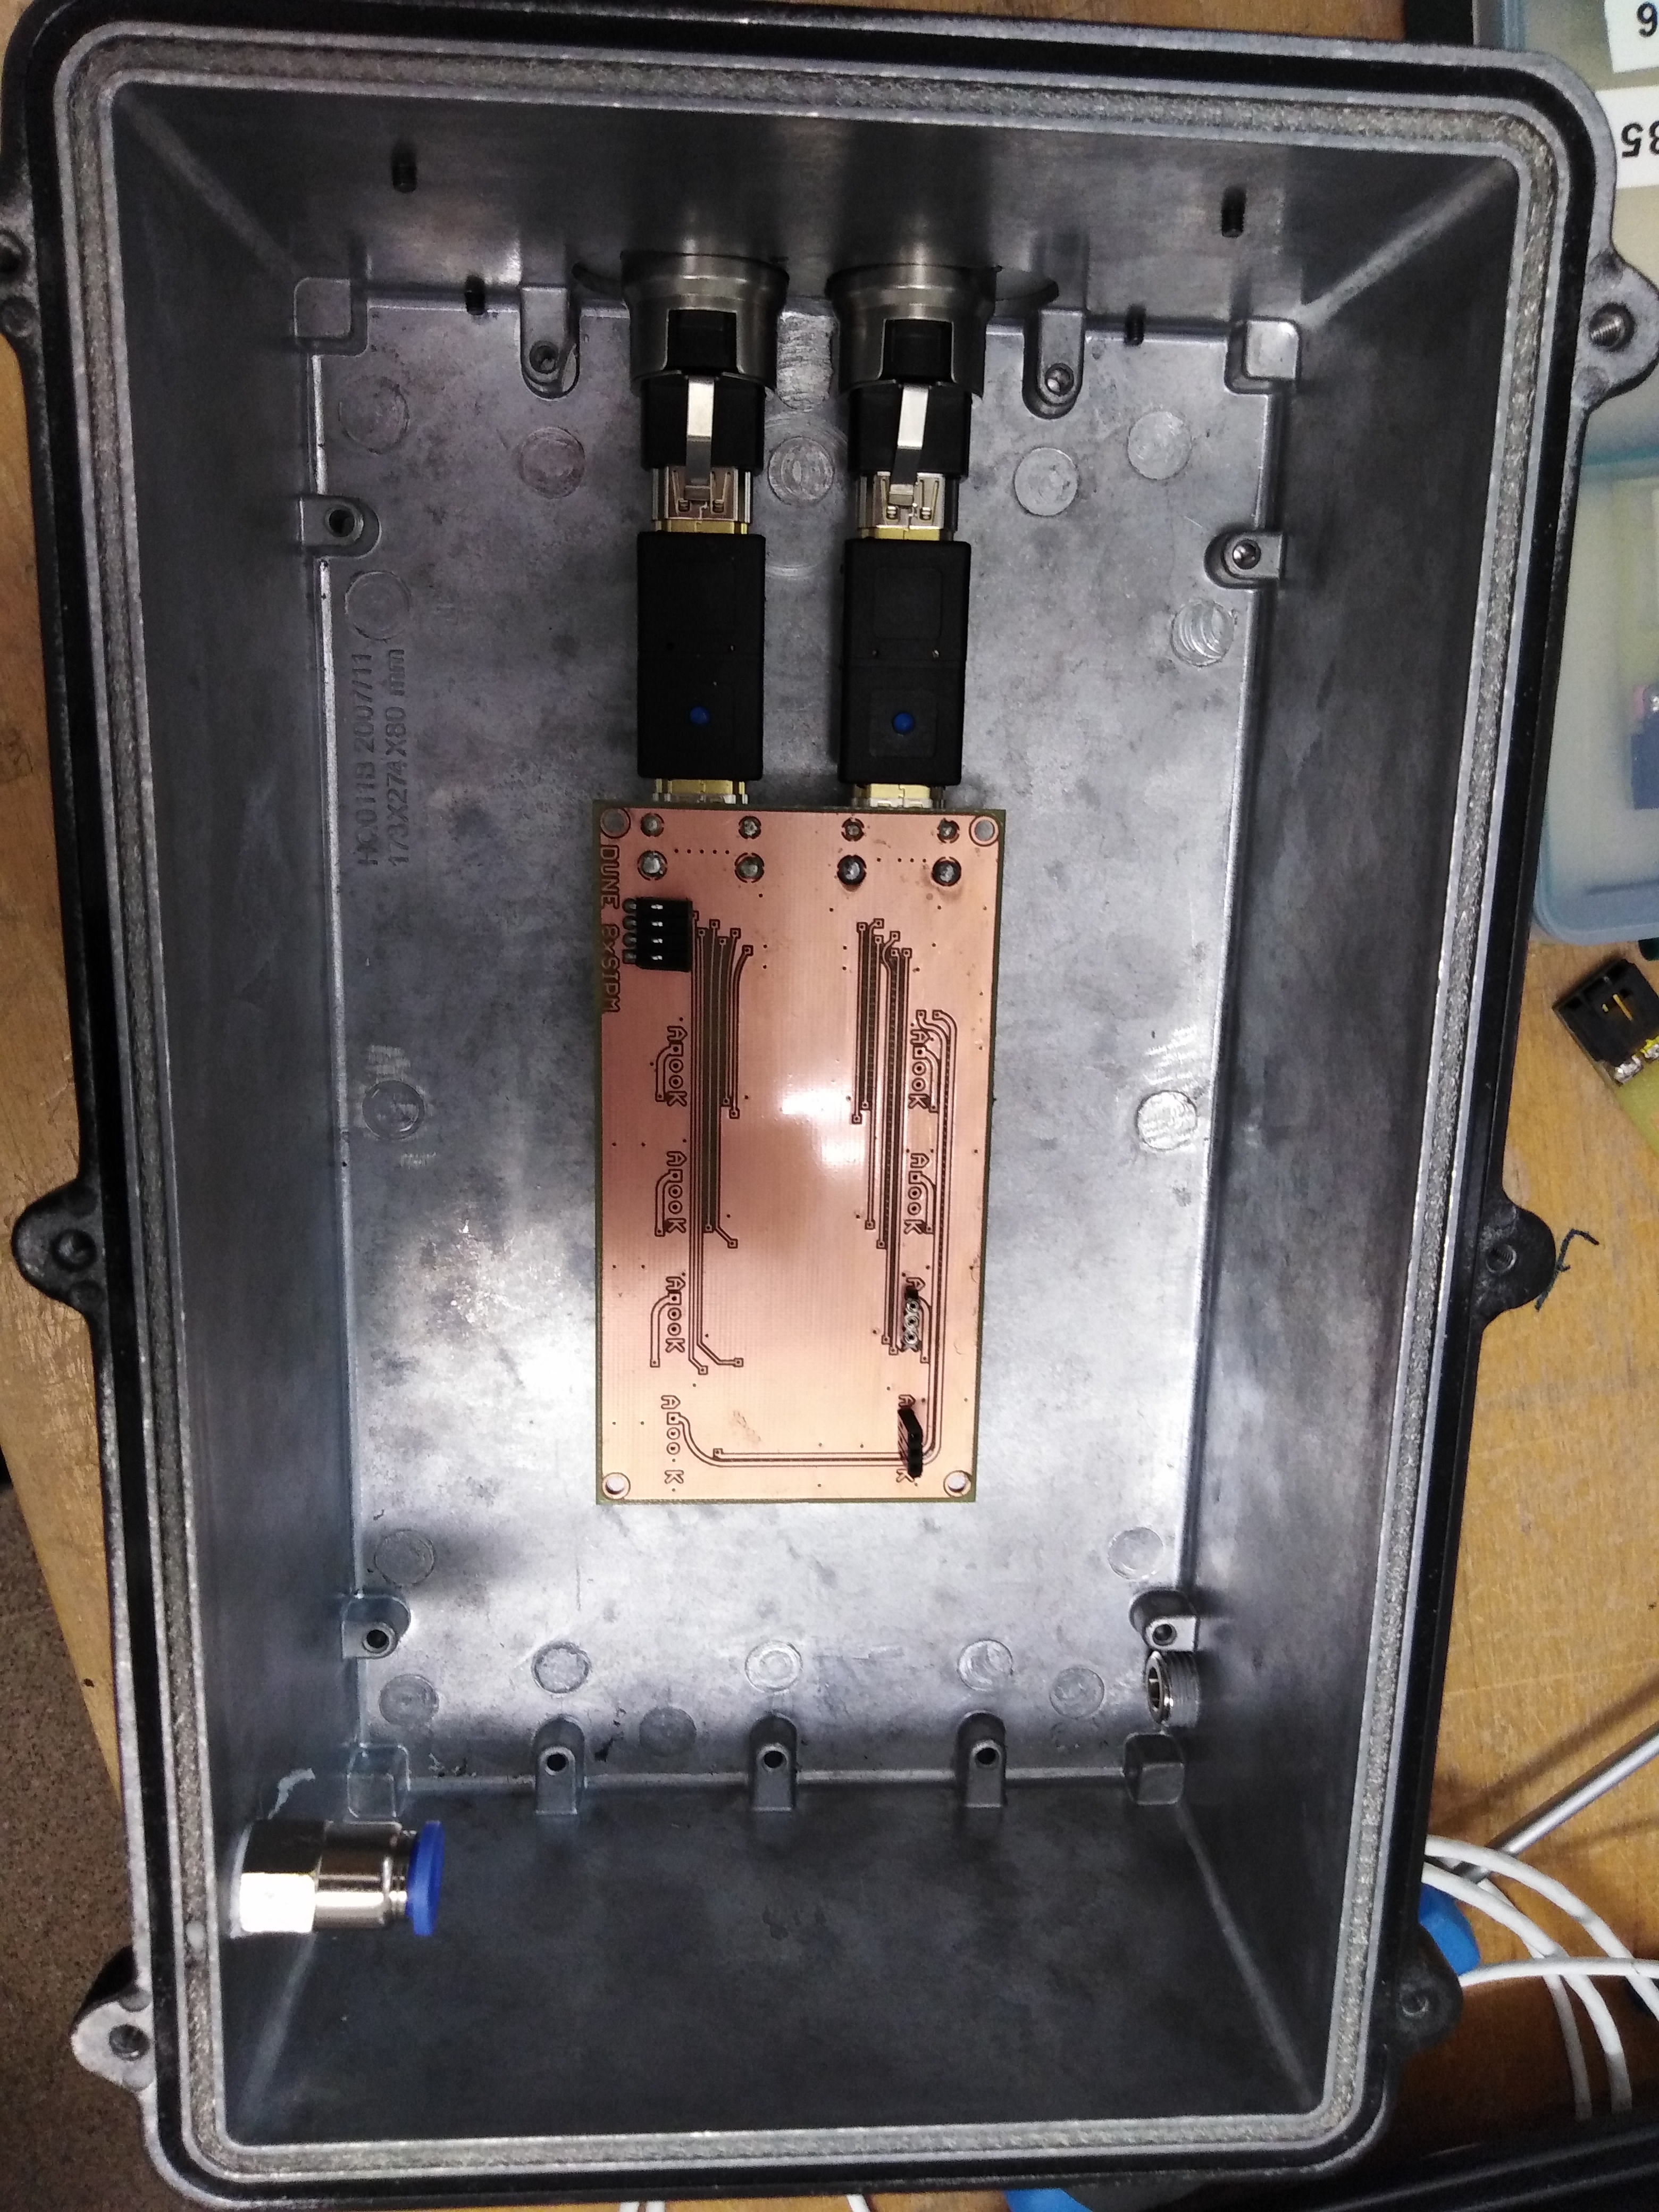
\includegraphics[scale=0.1]{3DesignPrinciples/32Tritium_detector/PCB1_SiPM_Black_Box.jpg}
\caption{The PCB 1 in which up to 8 SiPMs are connected inside the black box.\label{fig:PCB1}}
\end{figure}

\begin{figure}[h]
\centering
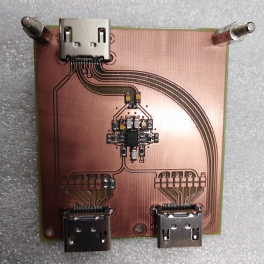
\includegraphics[scale=0.7]{3DesignPrinciples/32Tritium_detector/PCB2_SIPMs.png}
\caption{The PCB 2 in which the SiPMs output signals are summed and amplified.\label{fig:PCB2}}
\end{figure}

\begin{figure}[h]
\centering
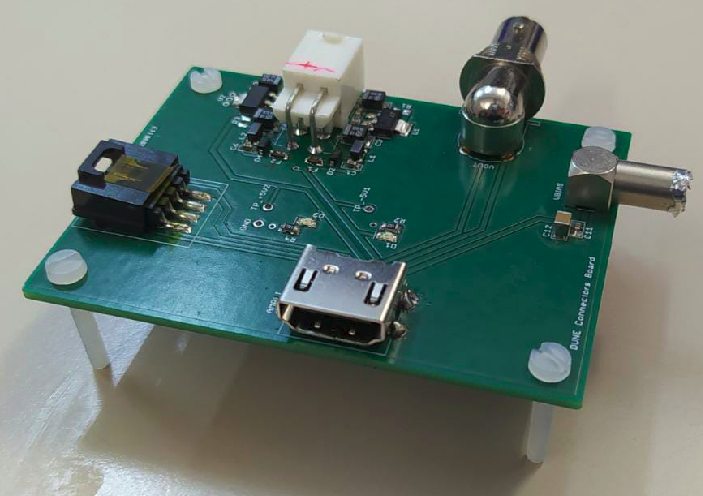
\includegraphics[scale=0.35]{3DesignPrinciples/32Tritium_detector/PCB3_SiPMs.png}
\caption{The PCB 3, in which the input and output signals of the system are rearranged.\label{fig:PCB3}}
\end{figure}

\begin{figure}[h]
\centering
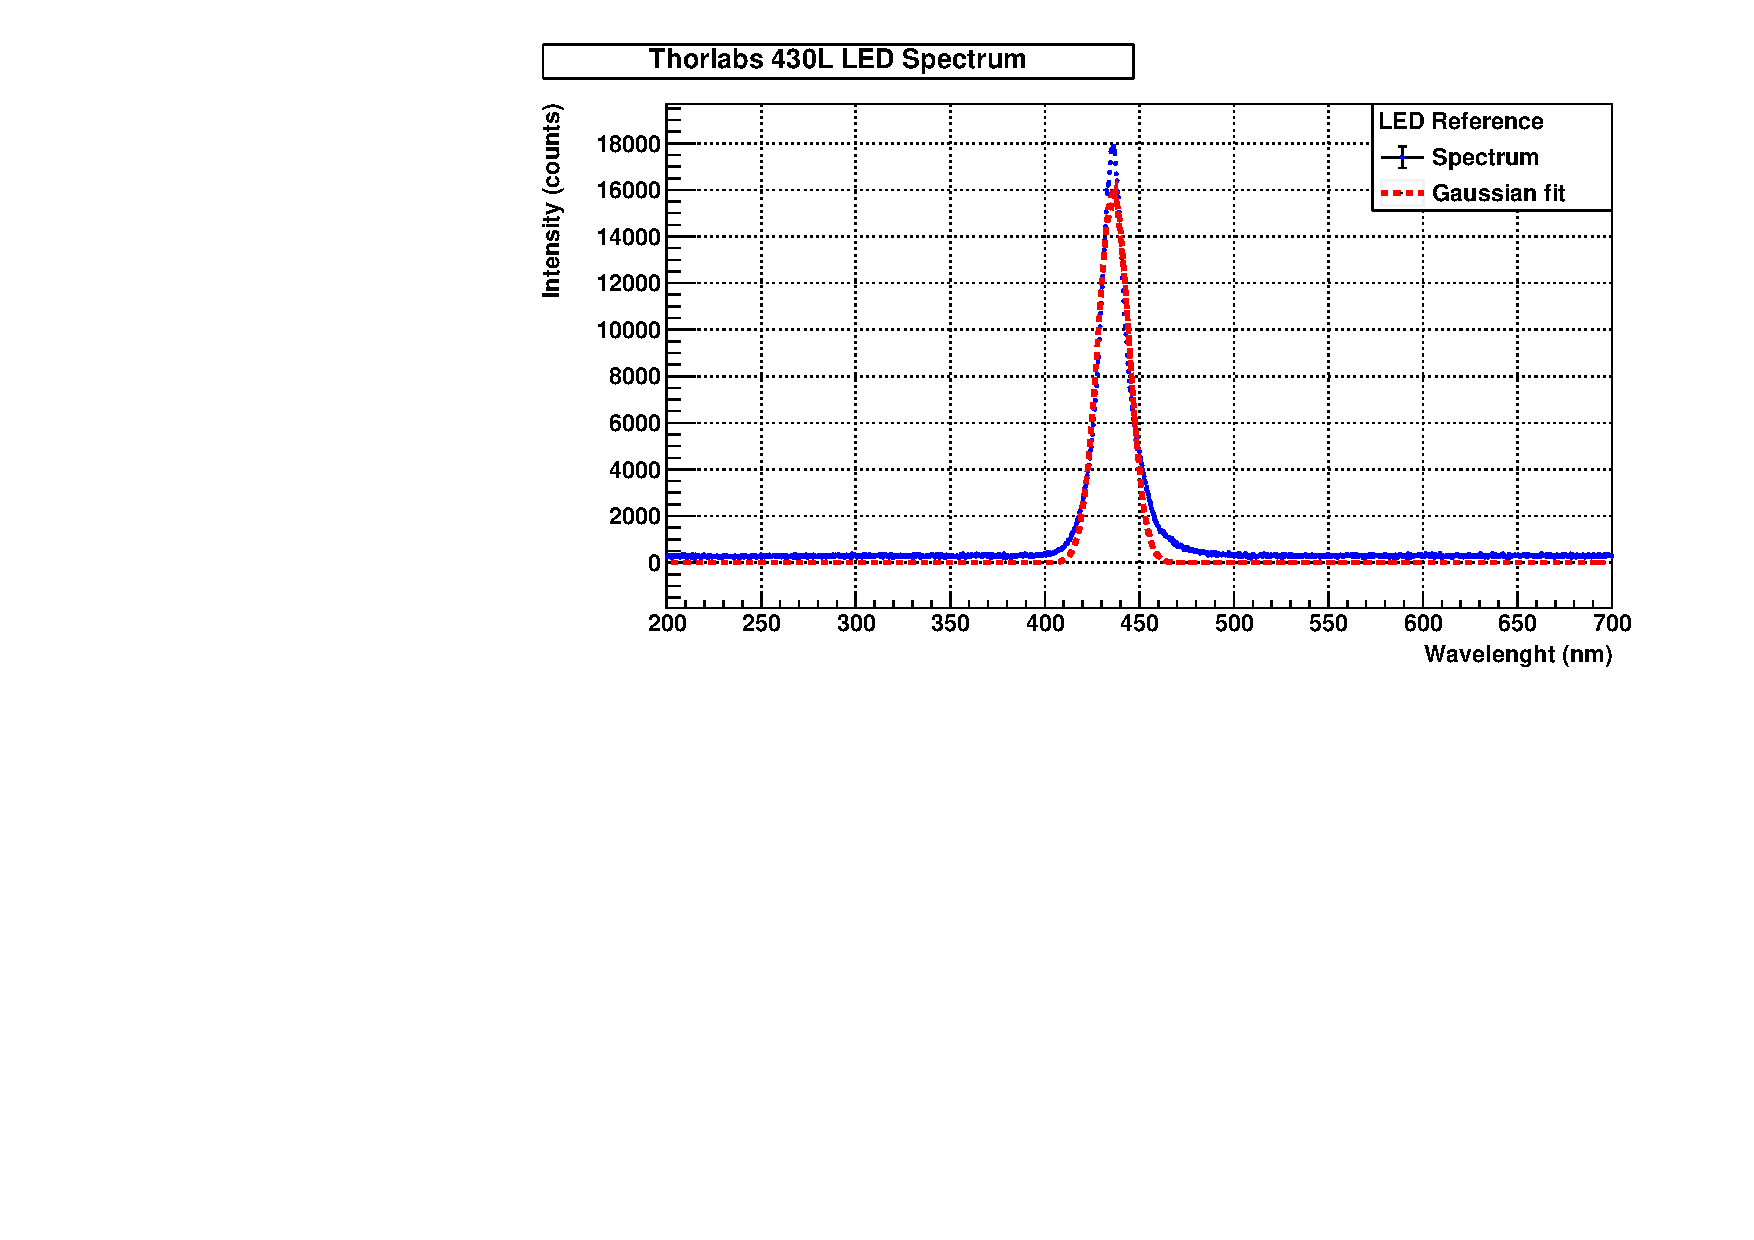
\includegraphics[scale=0.6]{3DesignPrinciples/32Tritium_detector/LED_DUNE.pdf}
\caption{The LED emission spectrum.\label{fig:LEDSpectrum}}
\end{figure}
